\documentclass[10pt,a4paper]{article}
%\usepackage{simplemargins}
\usepackage[margin=2.5cm]{geometry}
%\usepackage[square]{natbib}
\usepackage{amsmath}
\usepackage{amsfonts}
\usepackage{amssymb}
\usepackage{graphicx}
\usepackage{easyReview}
\usepackage{caption}

\begin{document}
	\pagenumbering{gobble}
	
	\Large
	\begin{center}
		Enhanced Pedestrian Dead Reckoning Sensor Fusion for Firefighting\\ 
		
		\hspace{10pt}
		
		% Author names and affiliations
		\large
		Tobias Augustin, Daniel Ossmann \\
		
		\hspace{10pt}
		
		\small  
		Munich University of Apllied Sciences HM\\
		\{tobias.augustin, daniel.ossmann\}@hm.edu\\
		
		
	\end{center}
	
	\hspace{10pt}
	
	\normalsize
	
	Knowing the firefighter's positions in a building during an indoor firefighting operation is crucial to improve firefighting efficiency and safety. Since GPS lacks the required accuracy in indoor environments, an alternative solution is demanded. Examples are radio or Wi-Fi triangulation or magnetic field mapping. However, first responders unique challenges call for an approach reliant solely on body-worn sensors. This is due to the fact, that a mapping or radio setup can not be performed in every building where a fire can occur. The so called Pedestrian Dead Reckoning (PDR) approach, estimates an individual's position relative to a starting point. PDR solutions utilize step-detection as their main means of position tracking. While step-detection produces accurate results during normal walking processes, during dynamic activities like crouching the accuracy is significantly reduced. In this paper we propose an approach that features an enhanced sensor data fusion algorithm to increase position estimation accuracy in various moving scenarios. The algorithm features an inertial measurement unit (IMU) based step-detection enhanced with a tracking camera as a secondary sensor. The measured velocity and position data is fused in an extended Kalman filter. To evaluate the quality of the enhanced sensor fusion algorithm, results from a verification campaign in a camera based, high precision measurement environment are presented. This environment allows a sub centimeter tracking resolution of an individuals position. With the enhanced sensor fusion, a mean error of less than $1\,\mathrm{m}$ can be achieved which is significantly lower than using step detection only.
	\vspace{1cm}
	
	\begin{minipage}[l]{0.47\textwidth}
		\hspace*{-0.5cm}
		\vspace{-2cm}
		\begin{center}
			
			%\vspace{-2.3cm}
			%\hspace{-0.5cm}
			\includegraphics[width=1\textwidth]{Bilder/schema1.png}
			
			\captionof{figure}{Schematic structure of the enhanced sensorfusion algorithm. The position data estimated by the Tracking Camera and the Step Detection Algorithm are the measurement inputs of the Kalman Filter}
		\end{center}
		
	\end{minipage}
	\hspace{1cm}
	\begin{minipage}[r]{0.4\textwidth}
		\hspace{-0.5cm}
		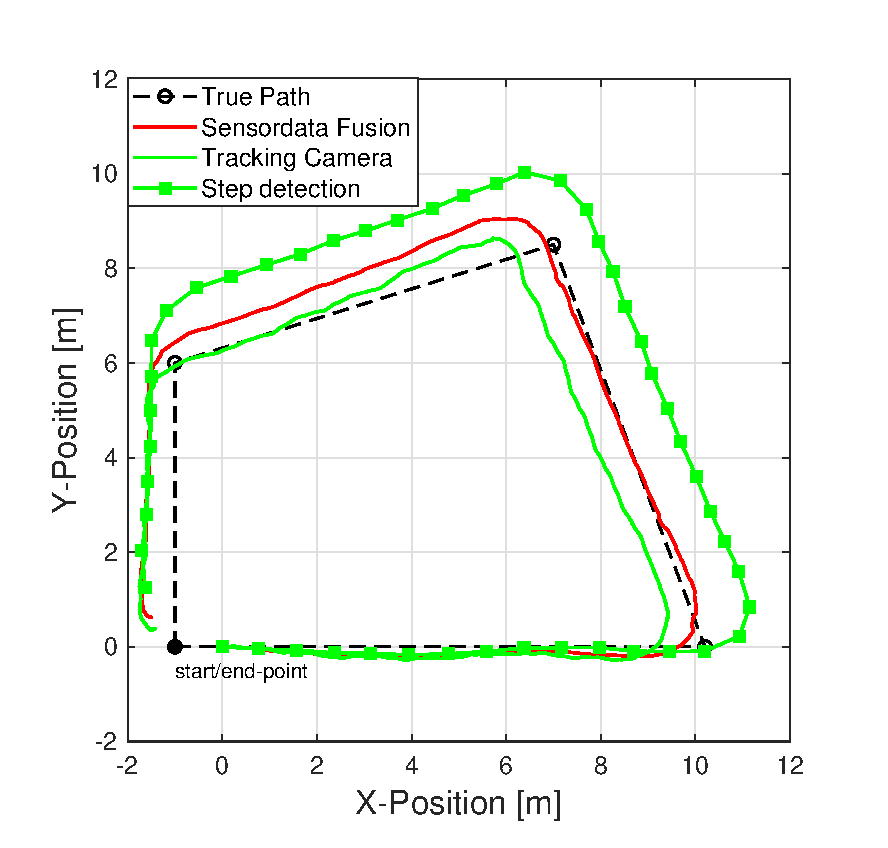
\includegraphics[width=1.2\textwidth]{Bilder/plotPaths.eps}
		
		\captionof{figure}{Comparison between Position Estimation based solely on a step length estimation algorithm or a Tracking Camera and the results estimated by the sensordata fusion algorithm.}
	\end{minipage}
	
\end{document}